\chapter{Approach and Implementation} % Main chapter title

\label{Chapter3} % For referencing the chapter elsewhere, use \ref{Chapter1} 

\lhead{Chapter 5. \emph{Approach and Implementation}}
\section{Approach}
To evaluate robustness of Selenium tests and to identify which factors contribute towards the robustness, a set of measurable metrics needs to be developed. This section introduces the rationale behind these metrics and highlights their significance.

\subsection{Robustness of Selenium tests}
\label{robustnessOfSeleniumTests}
Software development is a continuous and iterative process where an application undergoes through numerous changes. The commencing idea of this thesis is to assess whether Selenium tests are robust against these changes as the application evolves over time. As a starting point, it is essential to define the term \textit{robustness} within the context of Selenium testing. This section explains the notion behind robustness of Selenium tests and introduces the metric for measuring the robustness over different software revisions.

The purpose of test automation using Selenium framework is to spare the time and effort involved in executing regression tests manually every time the AUT changes. As mentioned in Chapter \ref{Chapter1}, such approach relies heavily on the robustness of underlying test-suite. Within the premise of this thesis, robustness of a Selenium test considers the degree of its stability and effectiveness to cover the intended functionality across different versions of the AUT. If a test is robust, it would ideally cover the same functionality across different revisions of the AUT and in cases where it fails, possible software \textit{regression} related to that functionality is found. In addition, a robust test also implies that it does not need to be constantly repaired as the AUT evolves. In practice, however, this characteristic may not always hold true since Selenium tests are built on top of the GUI layer of the application. Triggering certain behavior can involve multiple underlying functionalities and layers such as input validation, database operations etc.
% When the GUI of the application evolves over time, it usually evolves with other layers as opposed to changing in a standalone manner. As a result, the success of a test to cover the same functionality each time the application evolves depends on changes in other layers as well.
As an example, consider the \textit{click `Login' button} scenario from the \texttt{loginTest} in Listing \ref{code1}. If the new changes in AUT delays the time required for the GUI element locator of \textit{`Login'} button to be available in the DOM, the \texttt{loginTest} can fail randomly due to timing issues. Without specifying additional \texttt{wait} conditions in the test, desired functional coverage is not achieved and regression testing is likely to be ineffective. This rationale leads to the hypothesis that as the application evolves over time, the robustness of a test decreases and the test needs to be frequently repaired to maintain its robustness.  

% A test-suite is robust if it is able to cover the same functionality as the application changes over time.  

To evaluate how robust Selenium test \textit{T} is over time, it is possible to measure whether the test is able to cover the same functionality on different versions of AUT. As mentioned in Chapter \ref{Chapter2}, such a functionality coverage can be captured in terms of behavioral state models \cite{marchettoStateBased}, \cite{SchurMiningBehavModels}. If a test execution on different application versions results the same states of the behavioral model, such test can be considered robust.

This thesis proposes to measure the robustness of  \textit{T} for \textit{new version $V_{1}$} of the AUT against a \textit{reference version} \textit{$V_{0}$}. The \textit{reference version} of an application is the version for which the test \textit{T} is originally written and the states (functionalities) covered by \textit{T} are identified. The \textit{new version} correspond to iterative revisions of the application over time. The approach is straightforward -- the result of executing \textit{T} on reference version V$_{0}$ acts as a \textit{comparative oracle}, a benchmark against which performance of \textit{T} on new version V$_{1}$ can be measured. 

Formally, we define the term \textit{
robustness grade} to determine the robustness of test-suite T for test version V$_{1}$ compared against the reference version V$_{0}$. It can be calculated as follows:

% Robustness equation%

$$Robustness \thinspace Metric \thinspace (R_{T_{V_{0}V_{1}}}) = \displaystyle \frac{\#\thinspace of \thinspace same \thinspace states \thinspace reached \thinspace for \thinspace V_{1} \thinspace using \thinspace T}{\# \thinspace of \thinspace same \thinspace states \thinspace reached  \thinspace for \thinspace V_{0} \thinspace using \thinspace T}\normalsize$$

The robustness metric for a test version indicates the robustness of given test-suite and the functionality covered by it for that particular test version. The details of our approach to identify the state reached and functionalities covered across different versions are explained in Section XXX. As a starting point, we assume that the state extraction points for the reference version as well as subsequent versions remain the same as the test-suites remain unchanged. Correspondingly, if the tests written for the reference version cover the given functionalities as expected for the test version; the robustness metric for the test version (R$_{V_{0}V_{1}}$) is 100\%. A robustness metric of ‘100\%’ indicates that given tests are fully robust across these two versions and that they achieve similar behavioral state coverage. On the contrary, robustness metric less than 100\% deems that the given tests might not be fully robust. Such a metric indicates that these tests might be unable to cover the same application states or perhaps they trigger different application behavior for different versions. 

Our robustness measurement considers two kinds of versioning of the AUT: major versions (stable releases) where significant changes in functionality are done and minor revisions/commits where minor feature changes and bug fixes have been implemented.  In the first step we would measure the robustness metric for the major versions of the AUT to identify the changed functionality and perform the robustness analysis. Afterwards, for major versions with decreased robustness scores we plan to fix/modify the tests corresponding to the changed functionality for the subsequent major versions of the AUT. Second step would be to measure the robustness metric for the minor revisions of each major version to identify the regression changes. Our rationale behind this approach is that due to the significant functionality changes across the major versions, Selenium tests are less likely to fully cover the same behavioral states for all major versions unless they are modified. Utilizing the robustness scores for different versions of AUT we plan to investigate the reasons behind the varying robustness, and fix the broken Selenium tests in case of major versions. Further details about the robustness analysis  can be found in Section XXX
% In practice this is may not be the case, 
\texttt{==========================================================}

As described in Section \ref{testDesignPractices}, there are various \textit{building blocks} that compose a Selenium test. This composition can be broadly classified into UI locators, page-objects and \textit{actions} performed by the test. Depending upon how the test-suite is constructed, robustness of the tests can change -- as an example, consider number of state-changing \textit{actions} performed by the test. Recalling from Section \ref{sssec:emulatingActions}, a state-changing action such as a \textit{click} changes the DOM state. After this change, the page might not load all the elements of the DOM immediately -- which might cause interruption in the next action. In this manner, higher the number of state-changing actions a test executes, the more probability of it being fragile. Hence it would be interesting to know whether the composition of the test-suites affects the robustness of the tests. These factors are described in terms of measurable metrics in section \ref{robustnessFactors}.

Each GUI locator differs in their characteristics such as availability and their susceptibility towards changes in GUI structure. A structure dependent locator is likely to be broken by minor changes in the application's GUI and needs to be repaired repeatedly if the AUT has frequent GUI changes. This process adds additional overhead in terms of the time required and costs incurred with the maintenance of the test-suite. If developers know which locators are robust and do not need to be frequently repaired, they can improve their element location strategy to write more robust tests. Section \ref{locatorMaintenance} defines the metrics required to assess the maintenance effort for each locator type. 

\subsection{Factors affecting robustness of Selenium tests}
\label{robustnessFactors}
\subsection{Maintenance and repairing effort}
\label{locatorMaintenance}

\begin{figure}
\makeatletter 
\renewcommand{\thefigure}{\@arabic\c@figure}
\makeatother
% \setcounter{figure}{0}
    \centering
  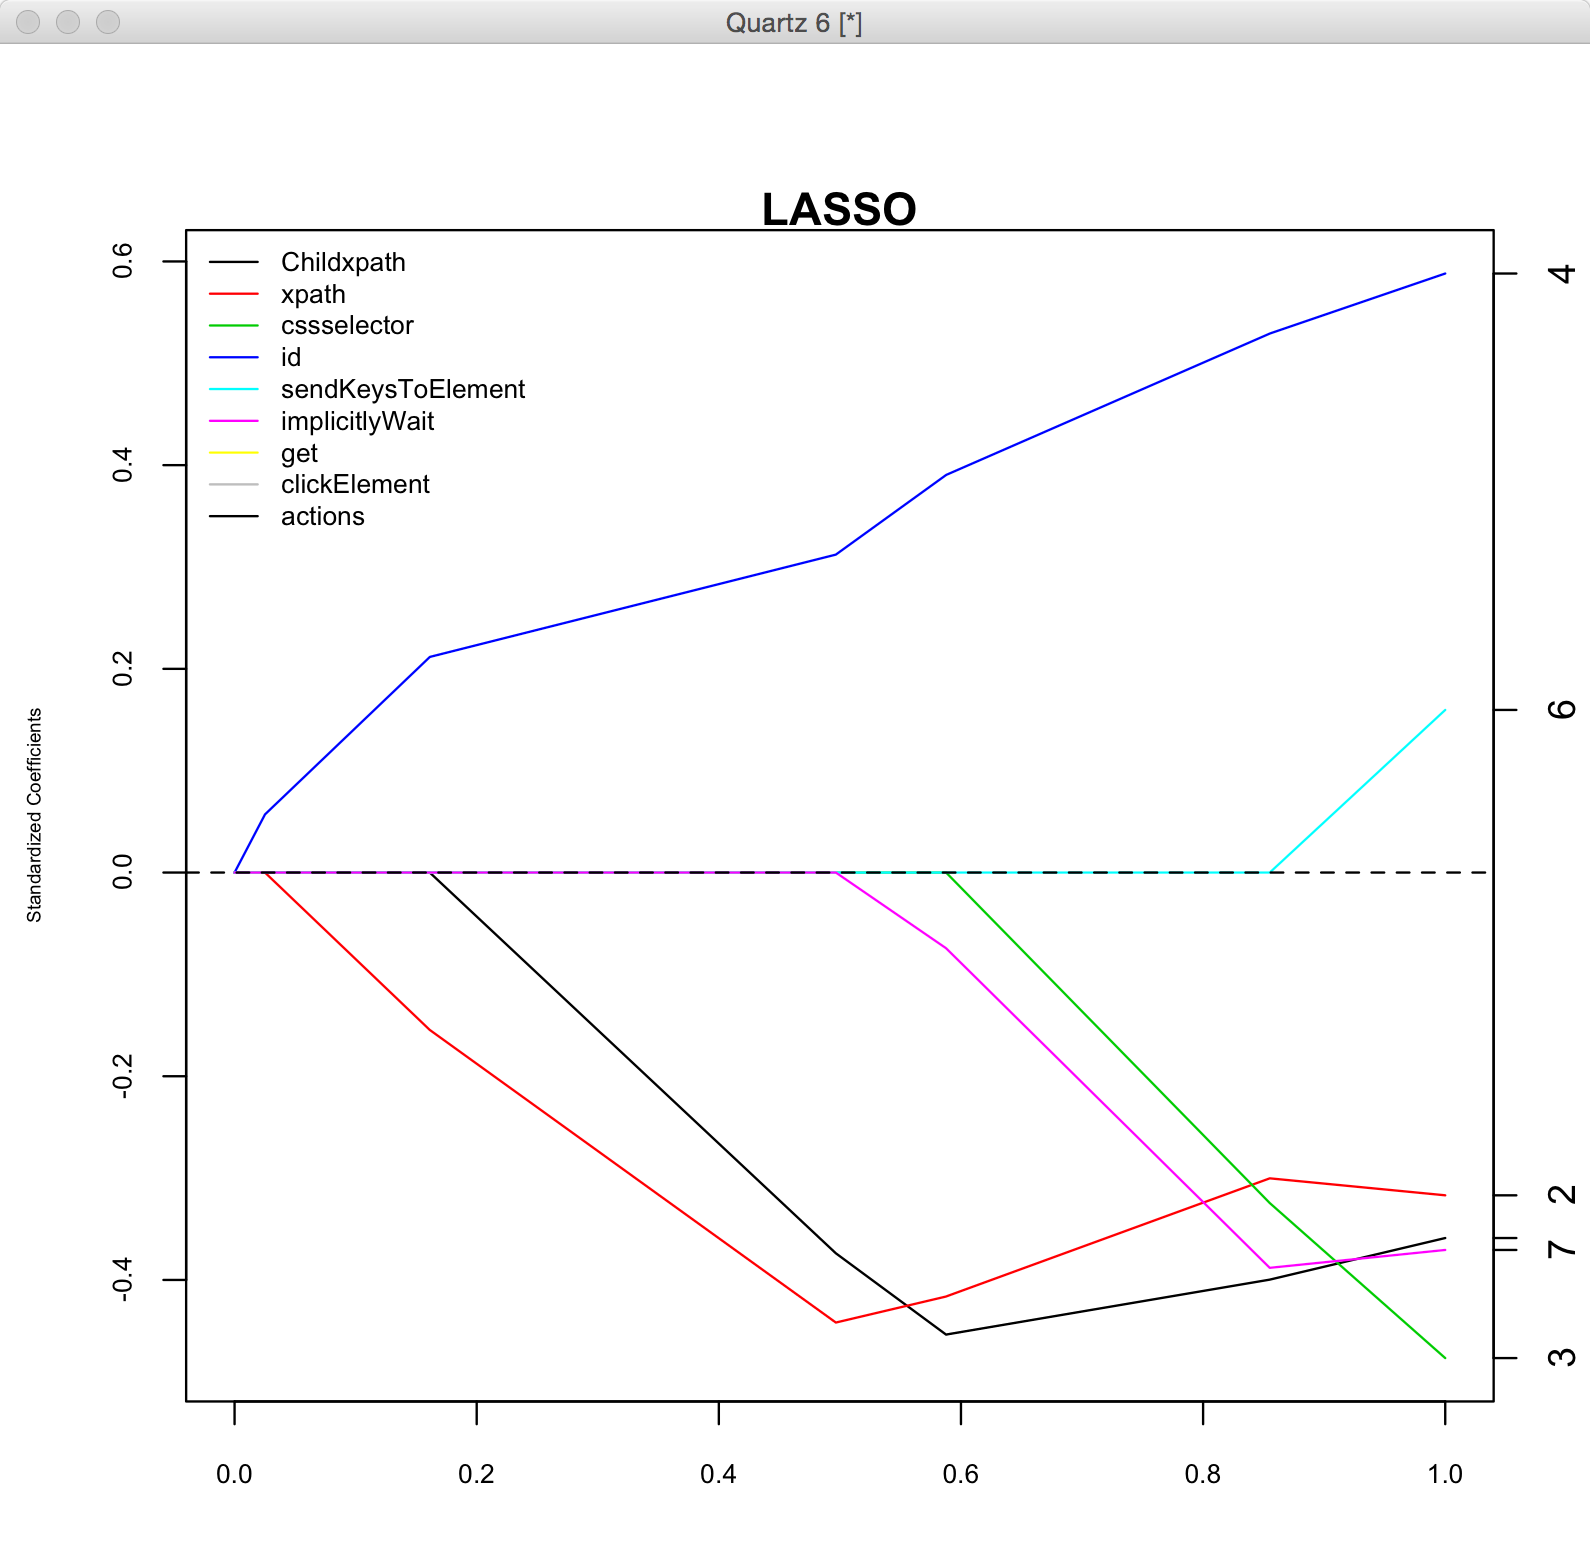
\includegraphics[width=4in,height=3.5in]{./Figures/lassotest.png}
  \caption{Lassotest}
  \label{fig:lassotest} 
\end{figure}

\begin{figure}
\makeatletter 
\renewcommand{\thefigure}{\@arabic\c@figure}
\makeatother
% \setcounter{figure}{0}
    \centering
  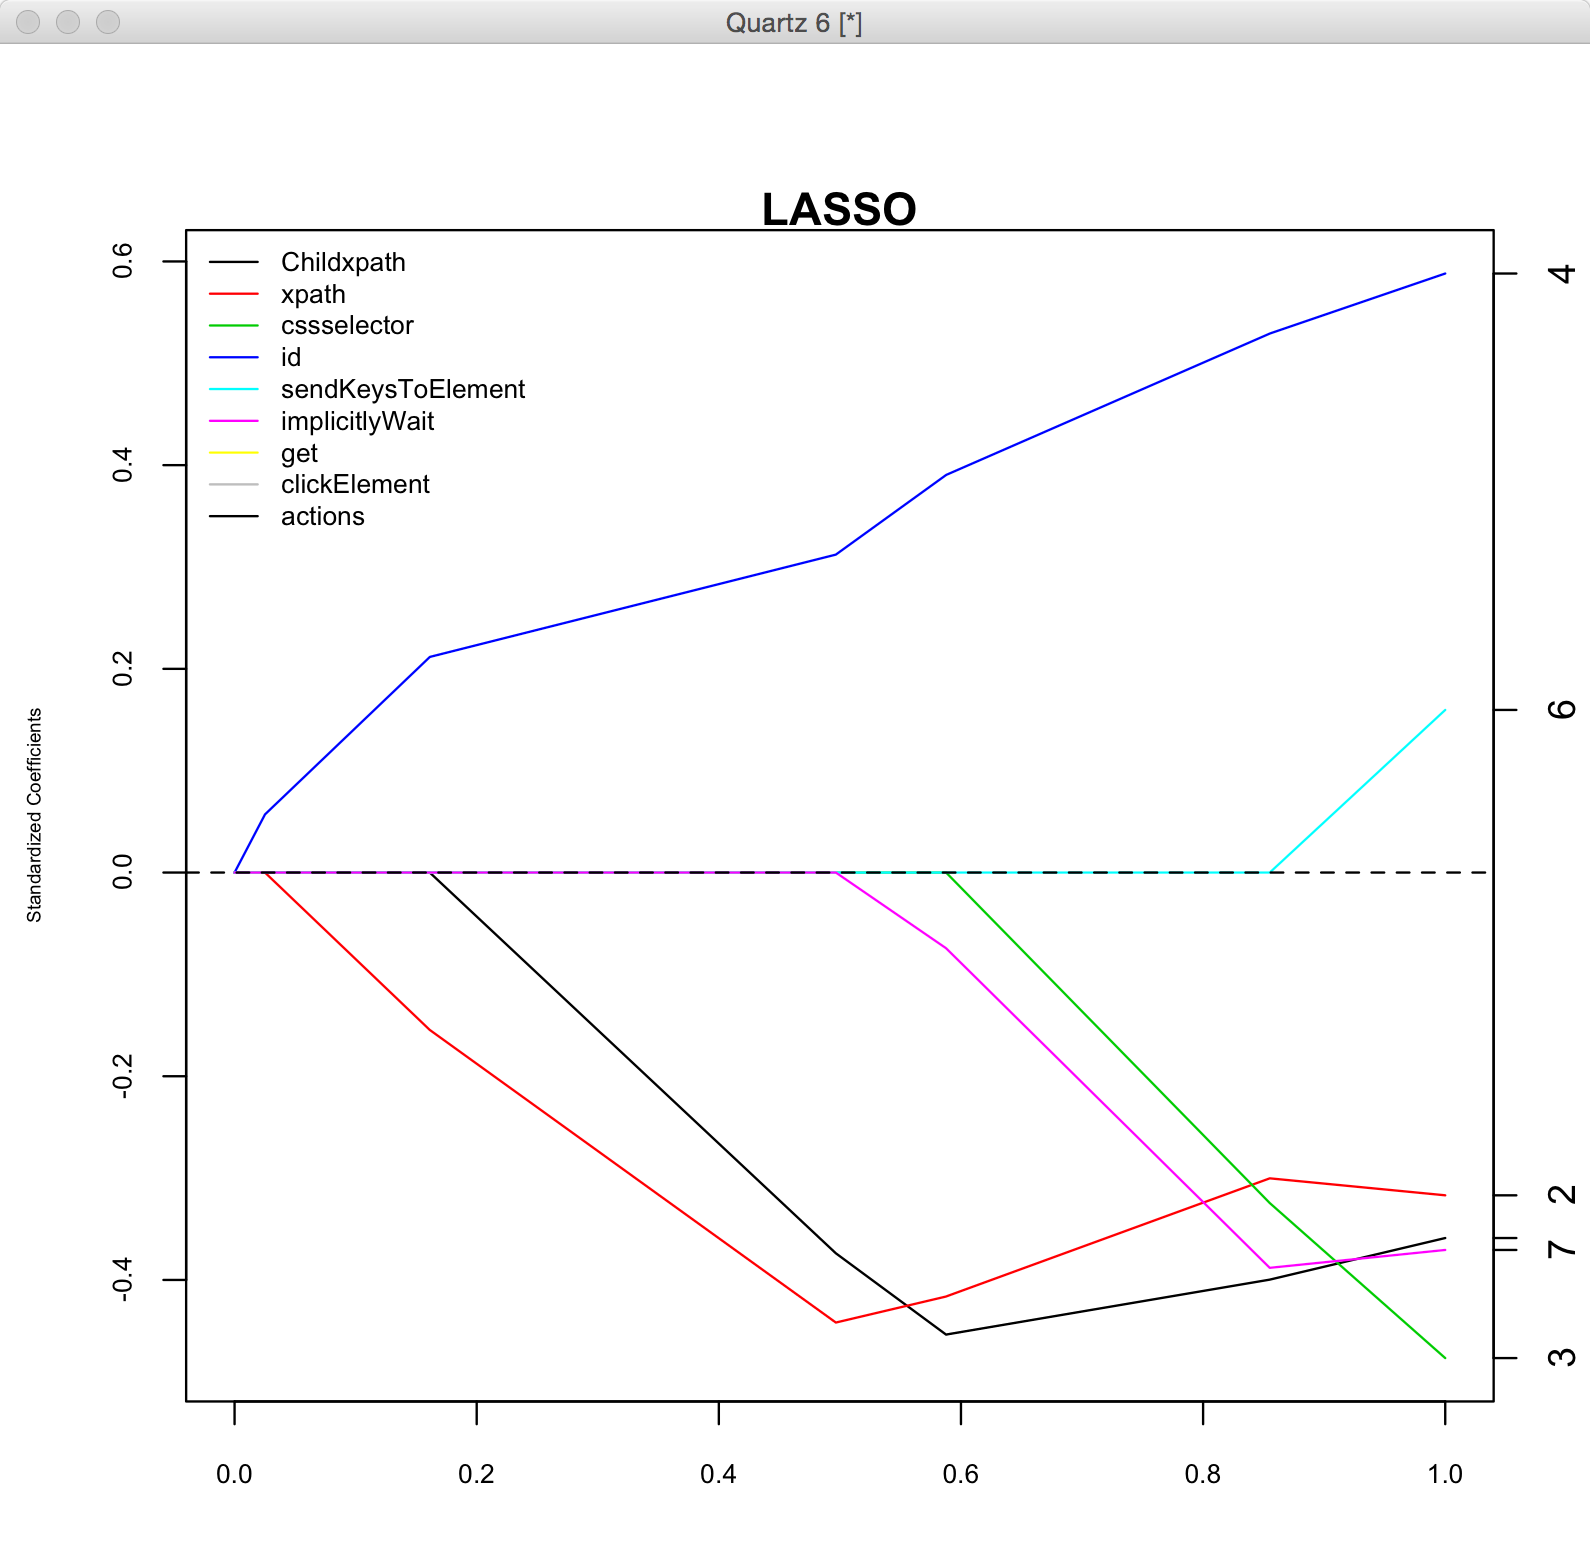
\includegraphics[width=3in,height=2.6in]{./Figures/lassotest.png}
  \caption{Lassotest}
  \label{fig:lassotest} 
\end{figure}
\begin{figure}
\makeatletter 
\renewcommand{\thefigure}{\@arabic\c@figure}
\makeatother
% \setcounter{figure}{0}
    \centering
  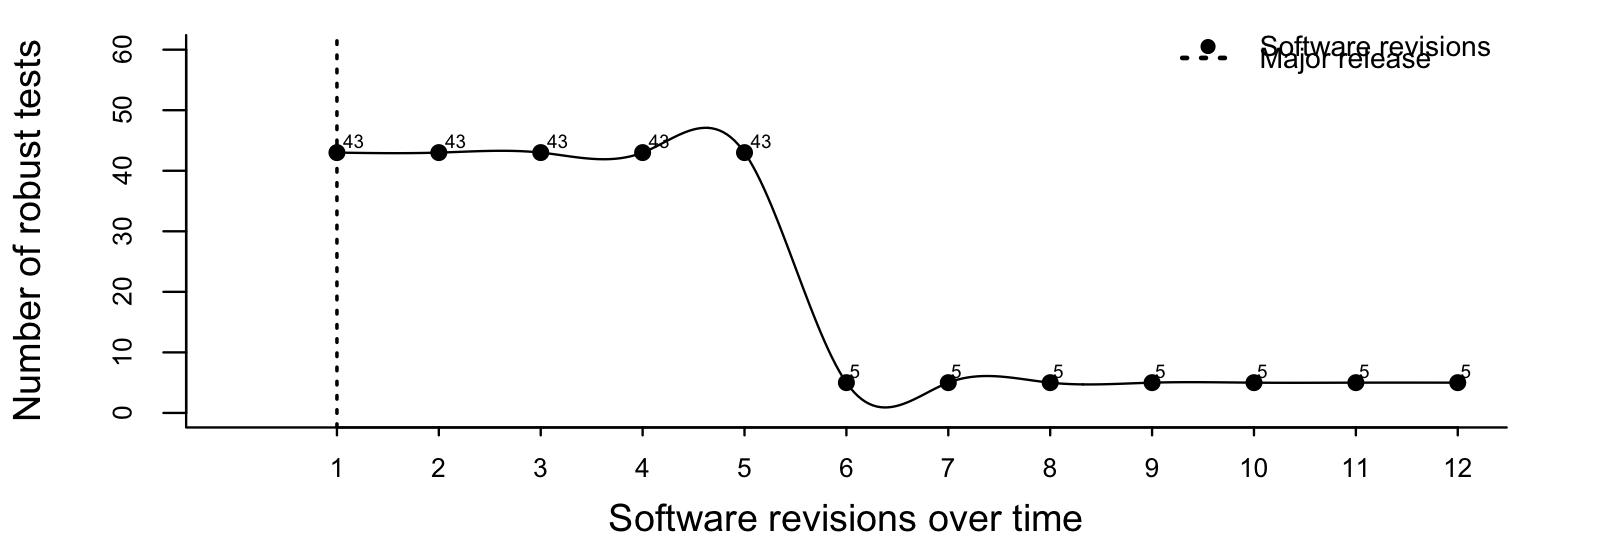
\includegraphics[width=6in,height=2.6in]{./Figures/moodlerq1pic.png}
\end{figure}
